%%%%%%%%%%%%%%%%%%%%%%%%%%%%%%%%%%%%%%%%%%%%%%%%%%%%%%%%%%%%%%%%%%%%%%%%%%
% ------------------------------------------------------------------------
% LaTeX FHPaper Template by Thomas MIGLINCI
% ------------------------------------------------------------------------
%
% Das eigentliche Paper beginnt ab Zeile 124 - dort die Daten in den
% Aufruf von FHInfo eintragen.
%
% Bitte ersetzen Sie gegebenenfalls Master-Studiengang Mechatronik/Robotik durch Bachelor-.....
%
% Erstellt von T. Miglinci, Jänner 2012 und getestet von W. Kubinger, März 2012 und September 2012
%
% Updates:
%  -) 30.10.2013, WK:
%
%%%%%%%%%%%%%%%%%%%%%%%%%%%%%%%%%%%%%%%%%%%%%%%%%%%%%%%%%%%%%%%%%%%%%%%%%%

\documentclass[10pt,a4paper,twoside]{article}

\usepackage{graphicx}
\usepackage[utf8]{inputenc}
\usepackage[T1]{fontenc}
\usepackage[english]{babel}

% mathematische Symbole
\usepackage{amsmath,amssymb,amsfonts,amstext}
%damit sind Bilder gezielter zu plazieren
\usepackage{float}

%%% ----------------------------------------------------------------------
\usepackage{color}
% Die Corporate Farben sind Blau (RGB 0/134/203), Grün (RGB 0/132/98) und Grau (RGB 98/107/113)
\definecolor{fhblue}{RGB}{0,134,203}
\newcommand\FHblue{\textcolor{fhblue}}
\definecolor{fhgruen}{RGB}{0,132,98}
\newcommand\FHgruen{\textcolor{fhgruen}}
\definecolor{fhgrau}{RGB}{98,107,113}
\newcommand\FHgrau{\textcolor{fhgrau}}

\unitlength1mm

% Zitierung im Harvard-Style
\usepackage{harvard}
\usepackage{url} %Darstellung von URLs erlauben
\citationstyle{dcu}  % für Zitate
\bibliographystyle{style/HarvardFHTWMR_V1_2e}% für Literaturverzeichnis
\citationmode{abbr}
\newcommand\citet{\citeasnoun}
\newcommand\citep{\cite}
% \citet(cootes01) -> Cootes (2001)
% \citep(cootes01) -> (Cootes, 2001)
\renewcommand{\harvardand}{\&}
%Deutsch (wahlweise mit DE)
\newcommand{\acessedthrough}{Verfügbar unter:}%Für URL-Angabe
\newcommand{\acessedthroughp}{Verfügbar durch:}%Für URL-Angabe (Geschützte Datenbank, Zugriff durch FH)
\newcommand{\acessedat}{Zugang am}%Für URL-Datum-Angabe
%Englisch (wahlweise mit EN)
%\newcommand{\acessedthrough}{Available at:}%Für URL-Angabe
%\newcommand{\acessedthroughp}{Available through:}%Für URL-Angabe (Geschützte Datenbank, Zugriff durch FH)
%\newcommand{\acessedat}{Accessed}%Für URL-Datum-Angabe
% bis hierher

% Seiten-Layout definieren
\usepackage[tmargin=14.5mm, bmargin=20mm, lmargin=20mm, rmargin=20mm,
            paper=a4paper,nofoot=true, nohead=true, noheadfoot=true]{geometry}

\usepackage{multicol}
\setlength{\columnsep}{7mm}

% weniger Warnungen wegen überfüllter Boxen
\tolerance = 9999
\sloppy

% Anpassung einiger Überschriften
\addto\captionsngerman
{
  \renewcommand\figurename{Abb.}
  \renewcommand\tablename{Tab.}
}

% Abbildungen, Gleichungen und Tabellen werden fortlaufend nummeriert
\renewcommand\thefigure{\arabic{figure}}
\renewcommand\thetable{\arabic{table}}
\renewcommand\theequation{\arabic{equation}}
\renewcommand\thesection{\arabic{section}.}
\renewcommand\thesubsection{\thesection\arabic{subsection}.}

\makeatletter
  % Überschriften neu definieren
  \renewcommand\section
  {
    \@startsection
    {section}{1}{0mm}      % für 'section', Ebene 1, 0mm Einzug
    {9pt} {6pt}            % Abstand darüber und darunter
    {\noindent\fontsize{10}{9pt}\scshape\textbf}%
  }

  \renewcommand\subsection
  {
    \@startsection
    {subsection}{2}{0mm}    % für 'subsection', Ebene 2, 0mm Einzug
    {9pt} {6pt}             % Abstand darüber und darunter
    {\noindent\fontsize{9}{9pt}\textbf}
  }
  \renewcommand\abstract[2]
  {
    \noindent\fontsize{9}{9pt}\textit{\textbf{Abstract—} #1}\\
    \noindent\fontsize{9}{9pt}\textit{\textbf{Keywords—} #2}
  }

  \newcommand\FHInfo[8]
  {
    \begin{multicols}{2}
      \fontsize{11}{14pt}
      \noindent{\textbf{\small Master-Studiengang Robotics Engineering}}\\
      {\fontsize{10}{20pt}
        \noindent \small FH Technikum Wien, Höchstädtplatz 6, A-1200 Wien\\
        \vspace{30pt}
      }
      \columnbreak
      \begin{figure}[H]
        \begin{flushright}
        \includegraphics[width=40mm,height=15mm,keepaspectratio=true]{#3}
        \label{fig:logo}
        \end{flushright}
      \end{figure}
    \end{multicols}
    \begin{center}
      \fontsize{12}{14pt}
      \noindent \textbf{\textsc {#4\\}}
      \bigskip
      {\fontsize{10}{12pt}
        \noindent{\textbf{Student: } #5, \textbf{PK: } #6}\\
        \noindent{\textbf{Supervisor: } #7}\\
      }
    \end{center}
    \vspace{0mm}
  }
\makeatother


\begin{document}
  \pagestyle{empty}  % keine Kopf- oder Fusszeile

  \FHInfo
    {Eintrag wird nicht verwendet}              % Eintrag wird nicht verwendet
    {Eintrag wird nicht verwendet}              % Eintrag wird nicht verwendet
    {img/paper/FHTW_Logo_Farbe_randlos.jpg}                 % FH-Logo
    {Virtualization of a Real-Time Operating System for Robot Control \\
    with a Focus on Real-Time Compliance}                       % Titel der Arbeit
    {Pamuk, Halil Ibrahim, BSc.}            % Student-Name
    {51842568}                                    % Student-PK-Nr
    {Rauh, Sebastian, MSc. BEng.}            % Name FH-Betreuer (1. BegutachterIn)
    {Dr.nat.techn. Wöber, Wilfried, MSc.}            % Name Firmenbetreuer (2. BegutachterIn)

  \fontsize{9}{10pt}

  \begin{multicols}{2}
    \abstract{\textbf{Virtualizing real-time operating systems for robotic control offers many advantages over traditional hardware-based approaches, especially when it comes to flexibility, scaling, and costs. Virtualization addresses these issues but introduces overhead and latency. This thesis investigates the virtualization of a real-time operating system, which is built with Yocto, employs hard real-time through Xenomai 3 and is emulated using QEMU/KVM. The primary objective aim was to bridge the latency gap between virtualized and bare metal versions to ensure deterministic and reliable behavior, which is crucial for real-time robotics. Initial latency measurements showed a high gap between bare metal and virtualized setups. Extensive tuning across BIOS, kernel, host OS, QEMU/KVM, and Salamander 4 (guest) reduced worst-case latency from 707.622 µs to 17.134 µs, close to the bare metal performance of 10.709 µs. The improvement is validated using a robotic application, comparing tuned virtualization with untuned and hardware versions.}} {\textbf{Virtualization, Real-Time Systems, Latency Reduction, Robot Control}}

    \section{Introduction}
    \begin{figure}[H]
      \centering
      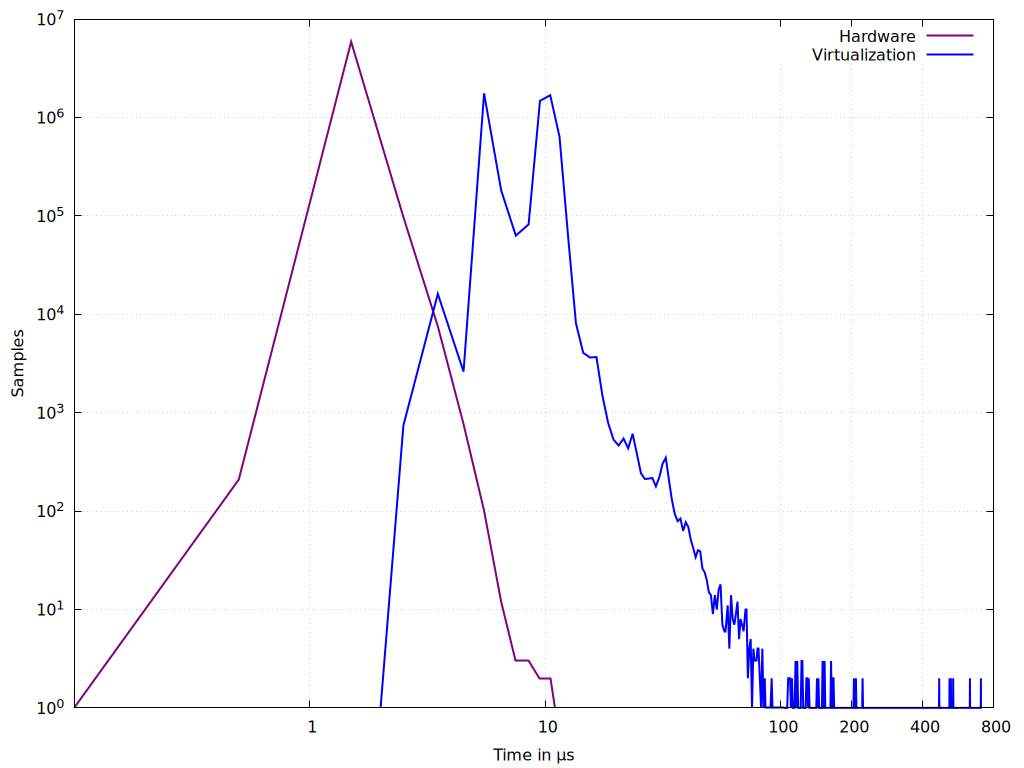
\includegraphics[width=1.0\columnwidth]{img/implementation/gnuplot_combined_max_latency.png}
      \caption[Initial Comparison of Latency Distribution between Hardware and Virtualization]{Initial Comparison of Latency Distribution between Hardware and Virtualization}
      \label{fig:gnuplot_max_latency_combined}
    \end{figure}

  
    \section{Methodology}
    \section{Implementation}
    \section{Initial Situation} 
    \section{Real-Time Performance Tunings}
    \section{Real-Time Robotic Application}
    \section{Results}
    \begin{figure}[H]
      \centering
      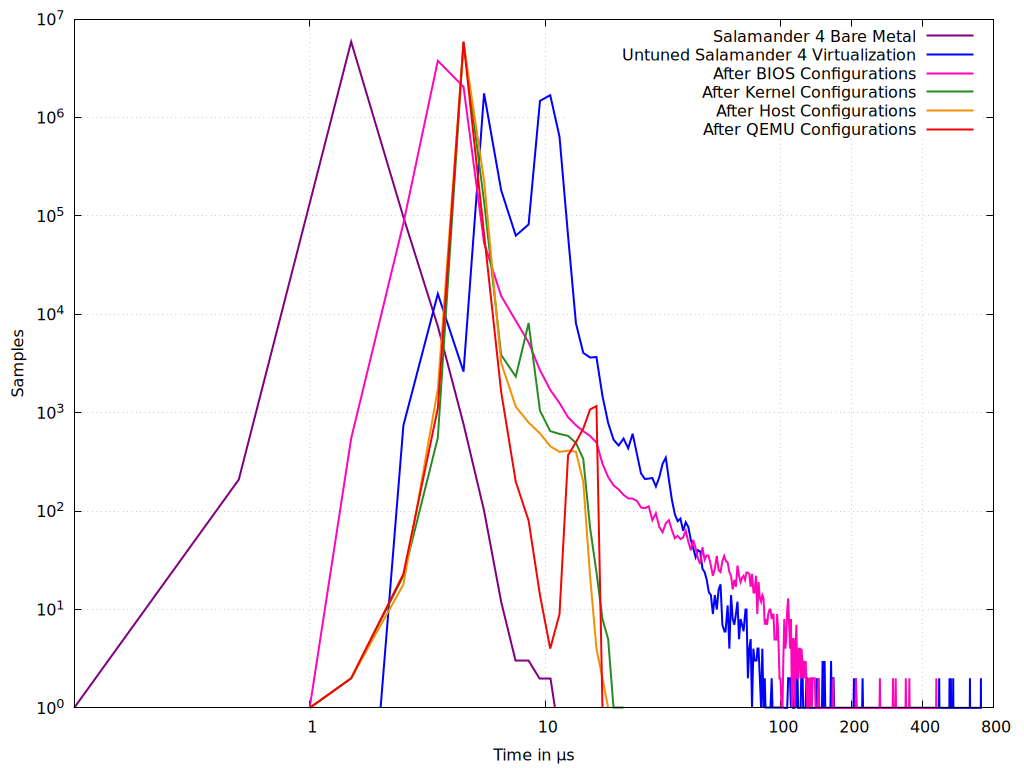
\includegraphics[width=1.0\columnwidth]{img/results/gnuplot_combined_max_latency_all.png}
      \caption[Comparison of Latency Distribution of Salamander 4 Configurations]{Comparison of Latency Distribution of Salamander 4 under different Configurations}
      \label{fig:max_latency_combined_results}
    \end{figure}

    \begin{figure}[H]
      \centering
      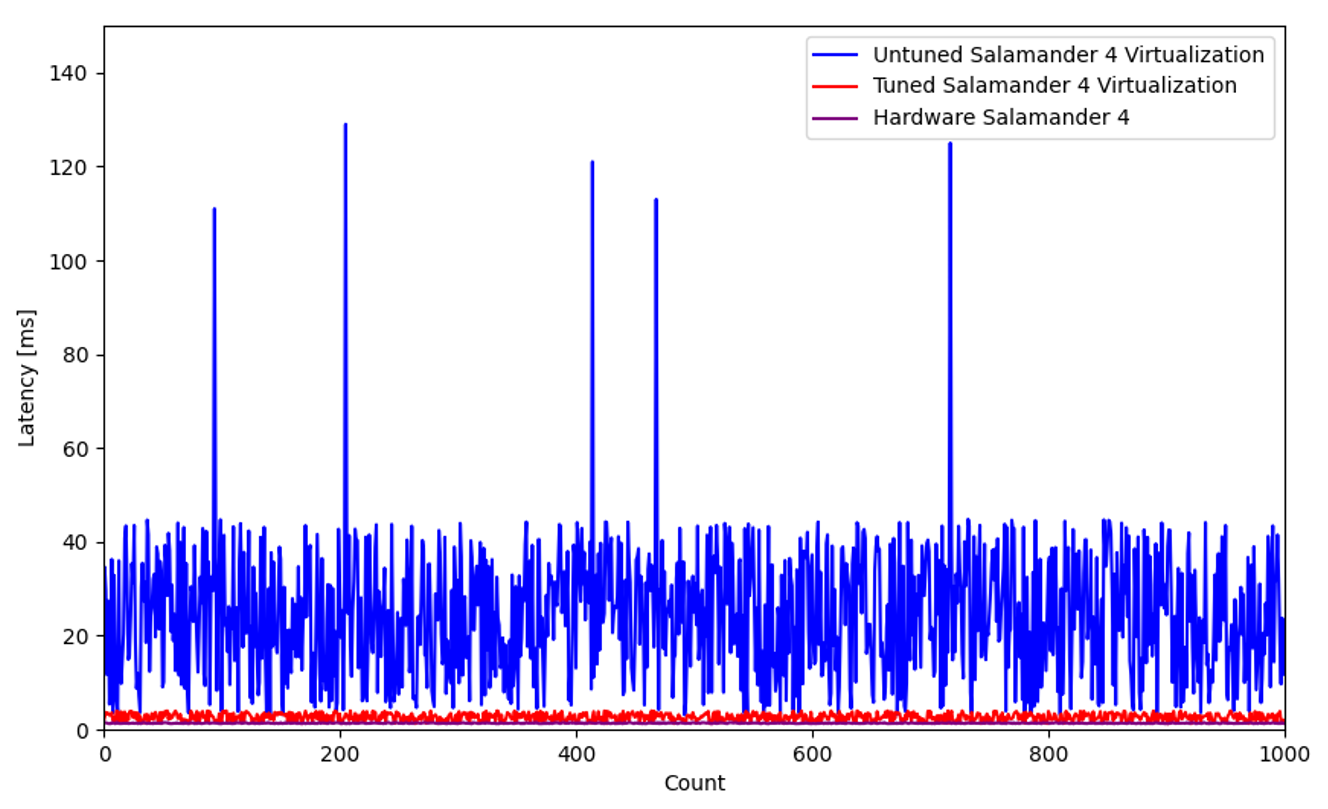
\includegraphics[width=1.0\columnwidth]{img/results/combined_latencies.png}
      \caption[Comparison of Robotic Application Latency of Salamander 4 Configurations]{Comparison of Robotic Application Latency of Salamander 4 under different Configurations}
      \label{fig:combined_latencies}
    \end{figure}

    
\begin{table}[H]
	\scriptsize
	\centering
	\caption{Comparison of Robotic Application Latency Statistics}
	\label{tab:robotic_application_latency_values_combined}
	\setlength{\tabcolsep}{0.5em} % for the horizontal padding
	{\renewcommand{\arraystretch}{1.2}% for the vertical padding
		\begin{tabular}{|l|l|l|l|l|l|}
			\hline
			\textbf{Tuning} & \textbf{Samples} & \textbf{Lat Min (ms)} & \textbf{Lat Avg (ms)} & \textbf{Lat Max (ms)} & \textbf{Std Dev (ms)} \\ \hline
			Hardware & 1000 & 1.211 & 1.347 & 1.49 & 0.082 \\ \hline
			Untuned Virtualization & 1000 & 3.1 & 24.603 & 129.46 & 13.876 \\ \hline
			Tuned Virtualization & 1000 & 1.219 & 2.62 & 3.988 & 0.812 \\ \hline
		\end{tabular}}
\end{table}

    \section{Discussion}
    \section{Summary and Outlook}
    Zusammenfassung stellt das Resümee und die kritische Reflexion über das Projekt dar.

    \section{Literaturverzeichnis}
    {
      \renewcommand{\refname}{\vspace{-5mm}} % keine eigene Überschrift durch \bibliography...
      \linespread{.8}\selectfont
      \bibliography{Literature_paper}
    }

  \end{multicols}

\end{document}
